%Correct the file name.
%X: book number
%Y: part number
%ZZZ: page number in three digits. So page 3 would be 003.

\documentclass[11pt]{amsbook}

\usepackage{../HBSuerDemir}	% ------------------------


\begin{document}

% ++++++++++++++++++++++++++++++++++++++
\hPage{b1p2/453}
% ++++++++++++++++++++++++++++++++++++++
\quad We establish the formula again for  $t_{n}$; the others are obtained similarly.
\begin{align*}
	I_{n} &= \int \! \tan^n \theta \, \hDif \theta \quad (n \ge 2) \\	
	&= \int \! \tan^{n-2} \theta tan^2 \theta \, \hDif \theta \\
	&= \int \! \tan^{n-2} \theta (\sec^2 \theta -1) \, \hDif \theta  \\
	&= \int \! \tan^{n-2} \theta \tan \theta - \int \! \tan^{n-2} \theta \, \hDif \theta\\
	&= \frac{1}{n-1} \tan^{n-1} \theta - I_{n-2} \\
\end{align*}
\begin{equation*}
 \left.\begin{aligned}
          		t_{n} &= -t_{n-2} + \frac{1}{n-1} \tan^{n-1} \theta \\
		t'_{n} &= -t'_{n-2}- \frac{1}{n-1} \cot^{n-1} \theta \\
	\end{aligned}
	 \right\}
 \qquad \text{}
\end{equation*}
 \begin{equation*}
 \left.\begin{aligned}
      		 T_{n} &= T_{n-2} - \frac{1}{n-1} \tanh^{n-1} \theta \\
		T'_{n} &= T'_{n-2} - \frac{1}{n-1} \coth^{n-1} \theta \\
       \end{aligned}
 \right\}
 \qquad \text{}
\end{equation*}
\begin{multicols}{2}
	\begin{align*}
		3.   c'_{n} &= \int \! \sec^{n} \theta \, \hDif \theta  \\
 		 s'_{n} &= \int \! \csc^{n} \theta \, \hDif \theta 
	\end{align*}

	\begin{align*}
		3'.  C'_{n} &= \int \! \text{sech}^{n} \theta \, \hDif \theta  \\
		S'_{n} &= \int \! \text{csch}^{n} \theta \, \hDif \theta 
	\end{align*}
\end{multicols}
Again we obtain the formula for $ c'_{n}$, the others being obtained similarly.
\begin{align*}
	c'_{n} &= \int \! \sec^{n} \theta \, \hDif \theta \quad (n \ge 2) \\
	&= \int \! \sec^{n-2}_{u} \theta \sec^{2}_{dv} \hDif \theta \\
	&= \sec^{n-2} \theta \tan \theta - \int \! \tan \theta . (n-2) \sec^{n-3} \theta \sec \theta \tan \theta \hDif \theta \\
	&= \sec^{n-2} \theta \tan \theta - (n-2) \int \sec^{n-2} \theta (sec^{2} \theta -1) \, \hDif \theta \\
	&= sec^{n-2} \theta \tan \theta - (n-2) c'_{n} + (n-2)c'_{n-2} \\
	(n-1)c'_{n} &= (n-2)c'_{n-2} + \sec^{n-2} \theta \tan \theta \\
	c_{n} &= \frac{n-2}{n-1} c'_{n-2} + \frac{1}{n-1} \sec^{n-2} \theta \tan \theta
\end{align*}




% =======================================
%\section{aaaah}






% =======================================
%\subsection{bbb}





% =======================================
%\subsubsection{cccc}

%This is the first figure. 
%\begin{figure}[htb]
%	\centering
%	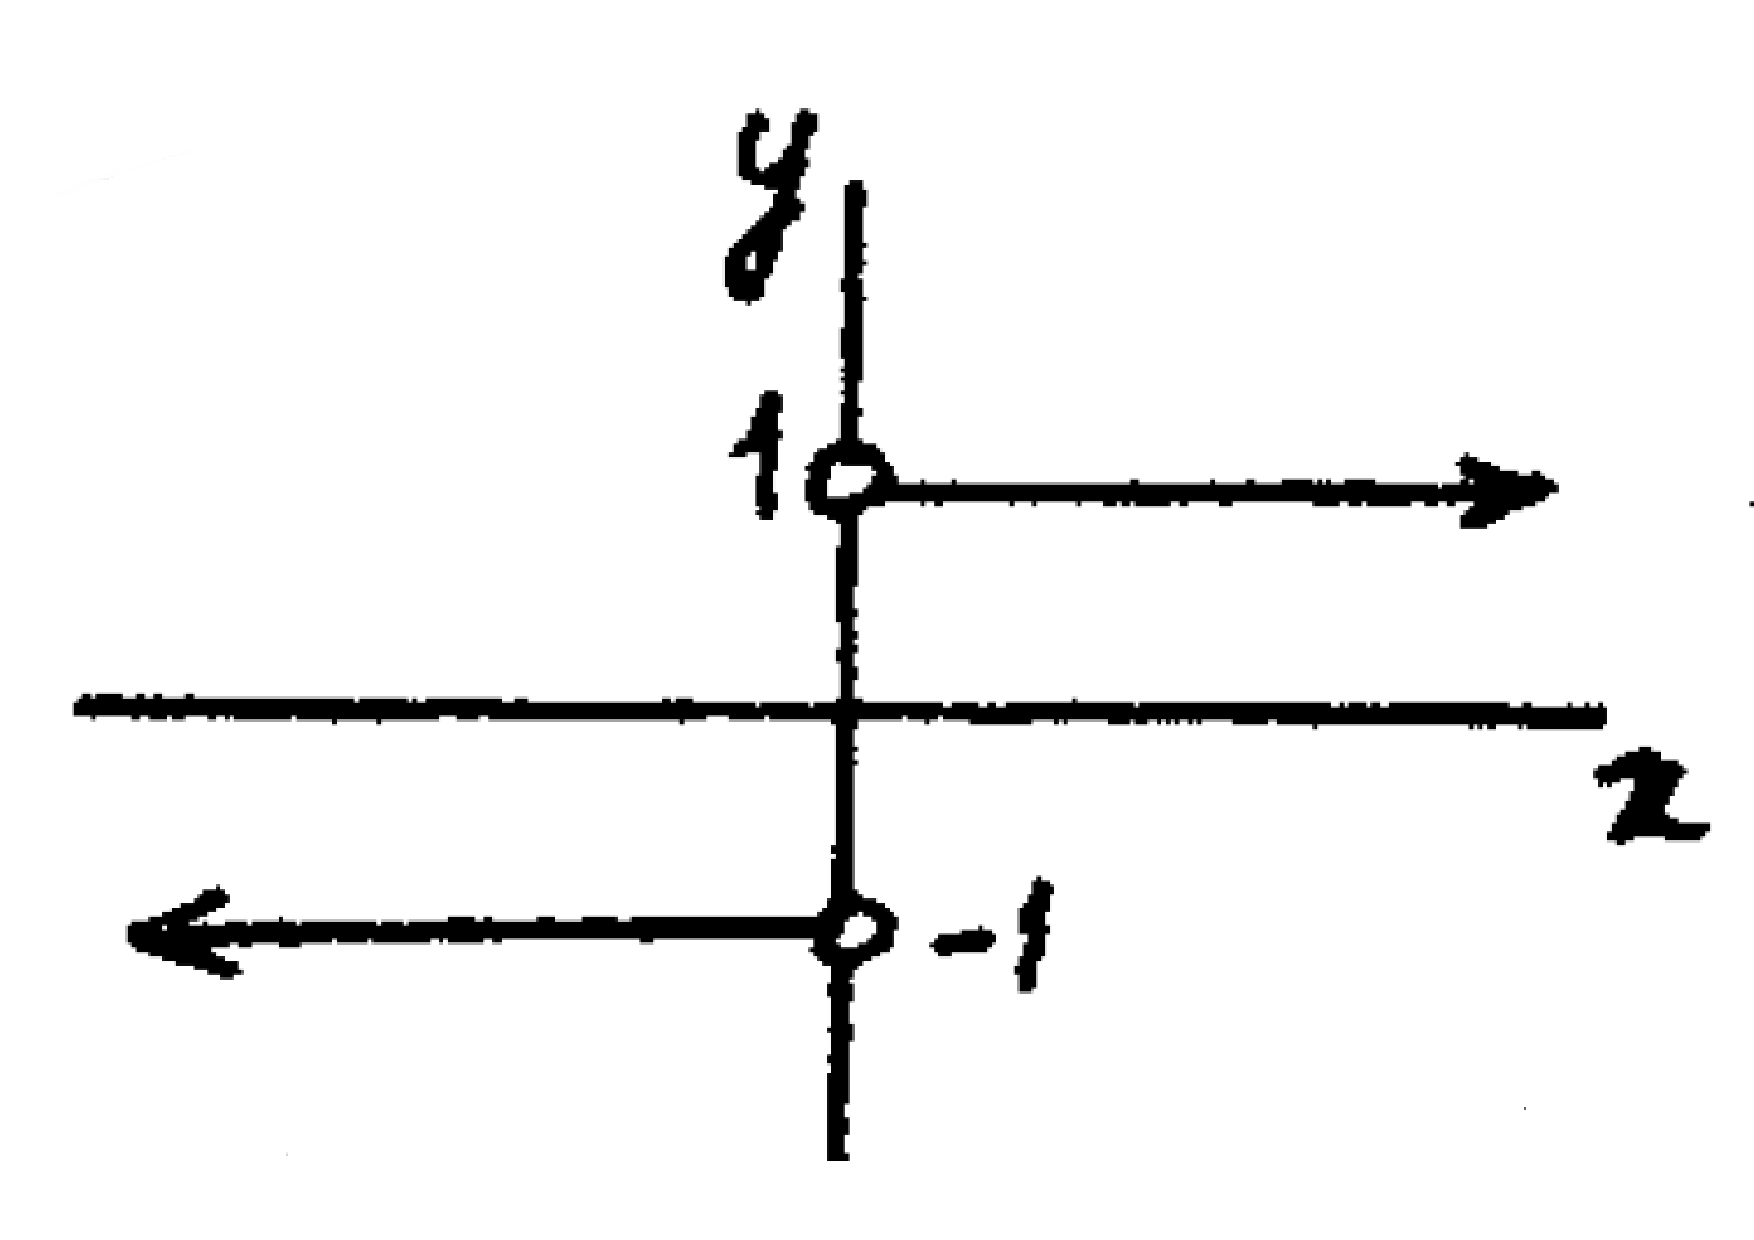
\includegraphics[width=0.45\textwidth]{images/bXpY-ZZZ-fig01}
%	\caption{Classification of complex numbers}
%	\label{fig:classificationOfComplexNumbersA}
%\end{figure}
%This is the second figure
%\begin{figure}[htb]
%	\centering
%	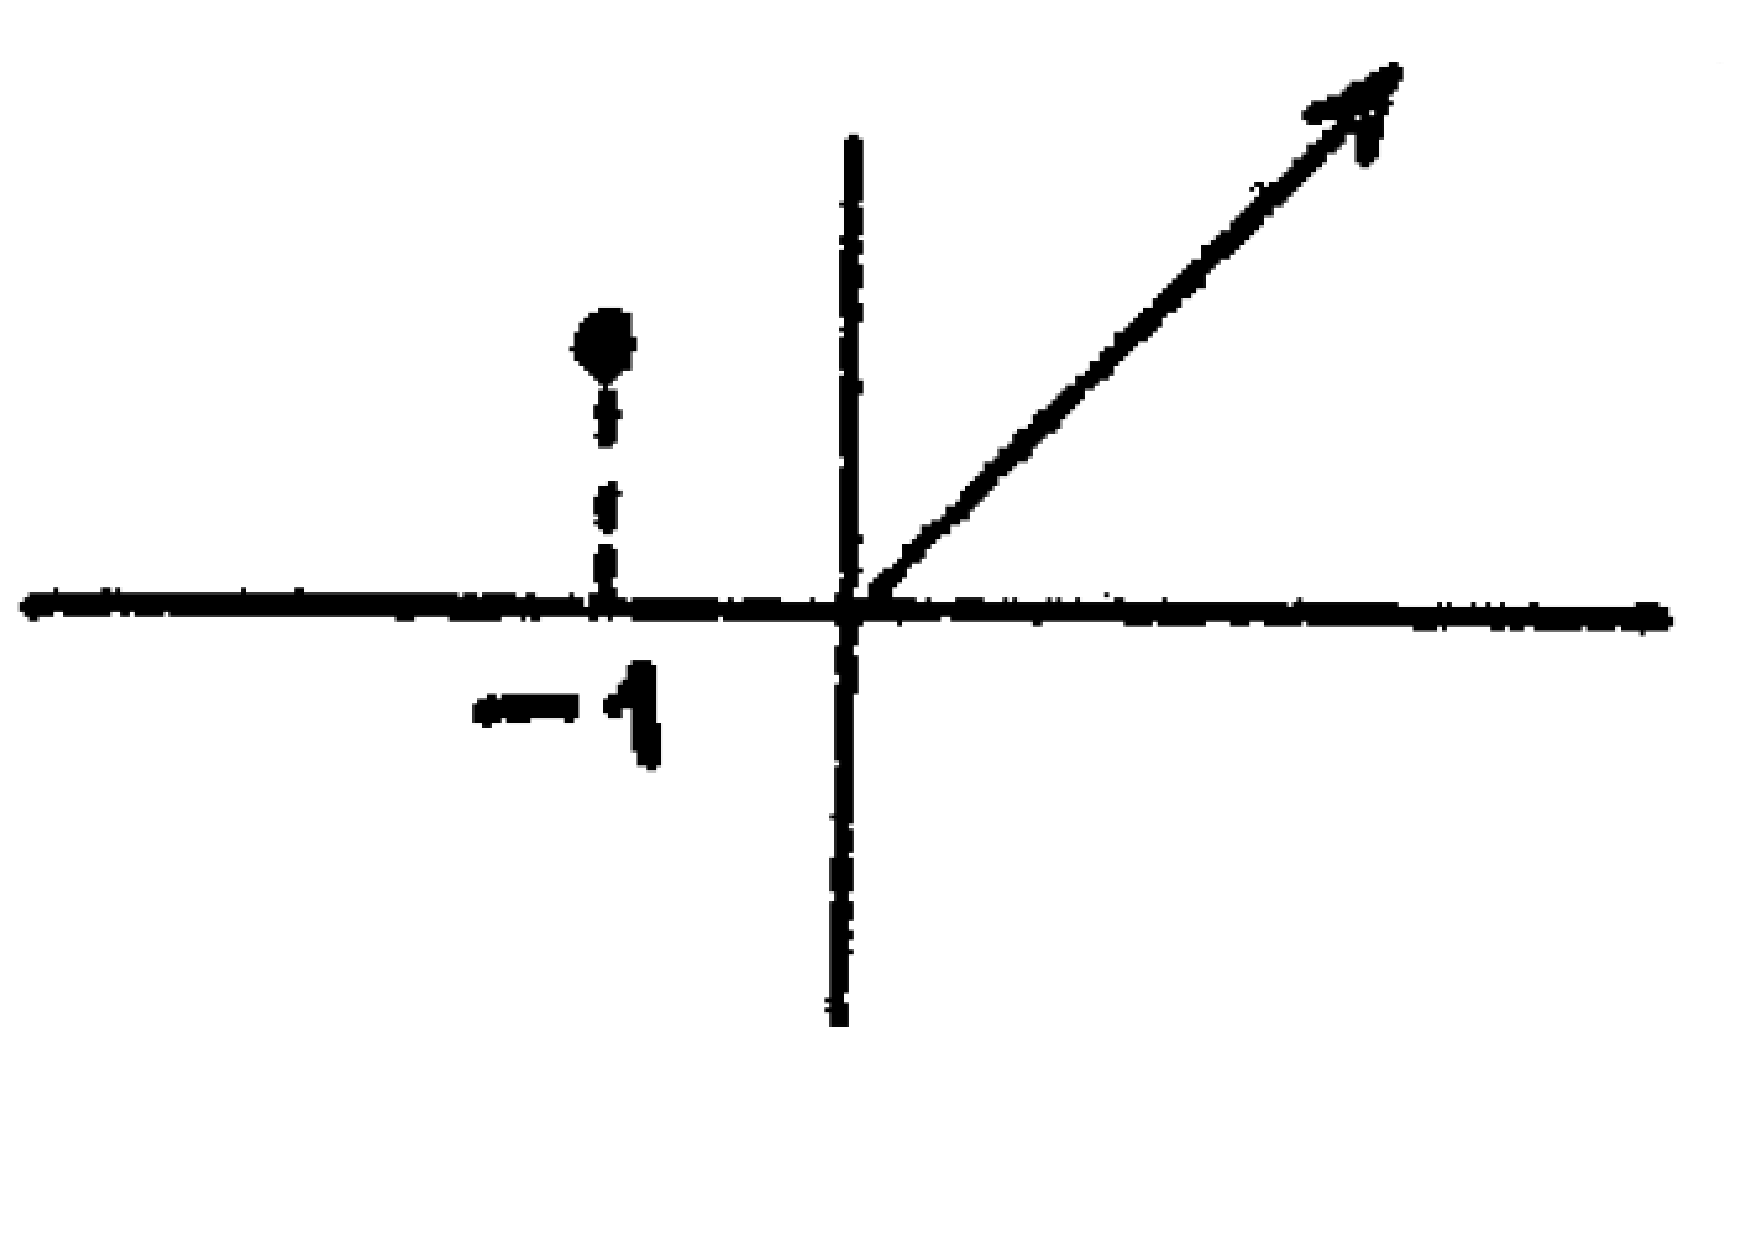
\includegraphics[width=0.45\textwidth]{images/bXpY-ZZZ-fig02}
%	\caption{Classification of complex numbers}
%	\label{fig:classificationOfComplexNumbersA}
%\end{figure}






% =======================================================
\end{document}  

%==== templates ====

%==== environments ====

%\begin{figure}[htb]
%	\centering
%	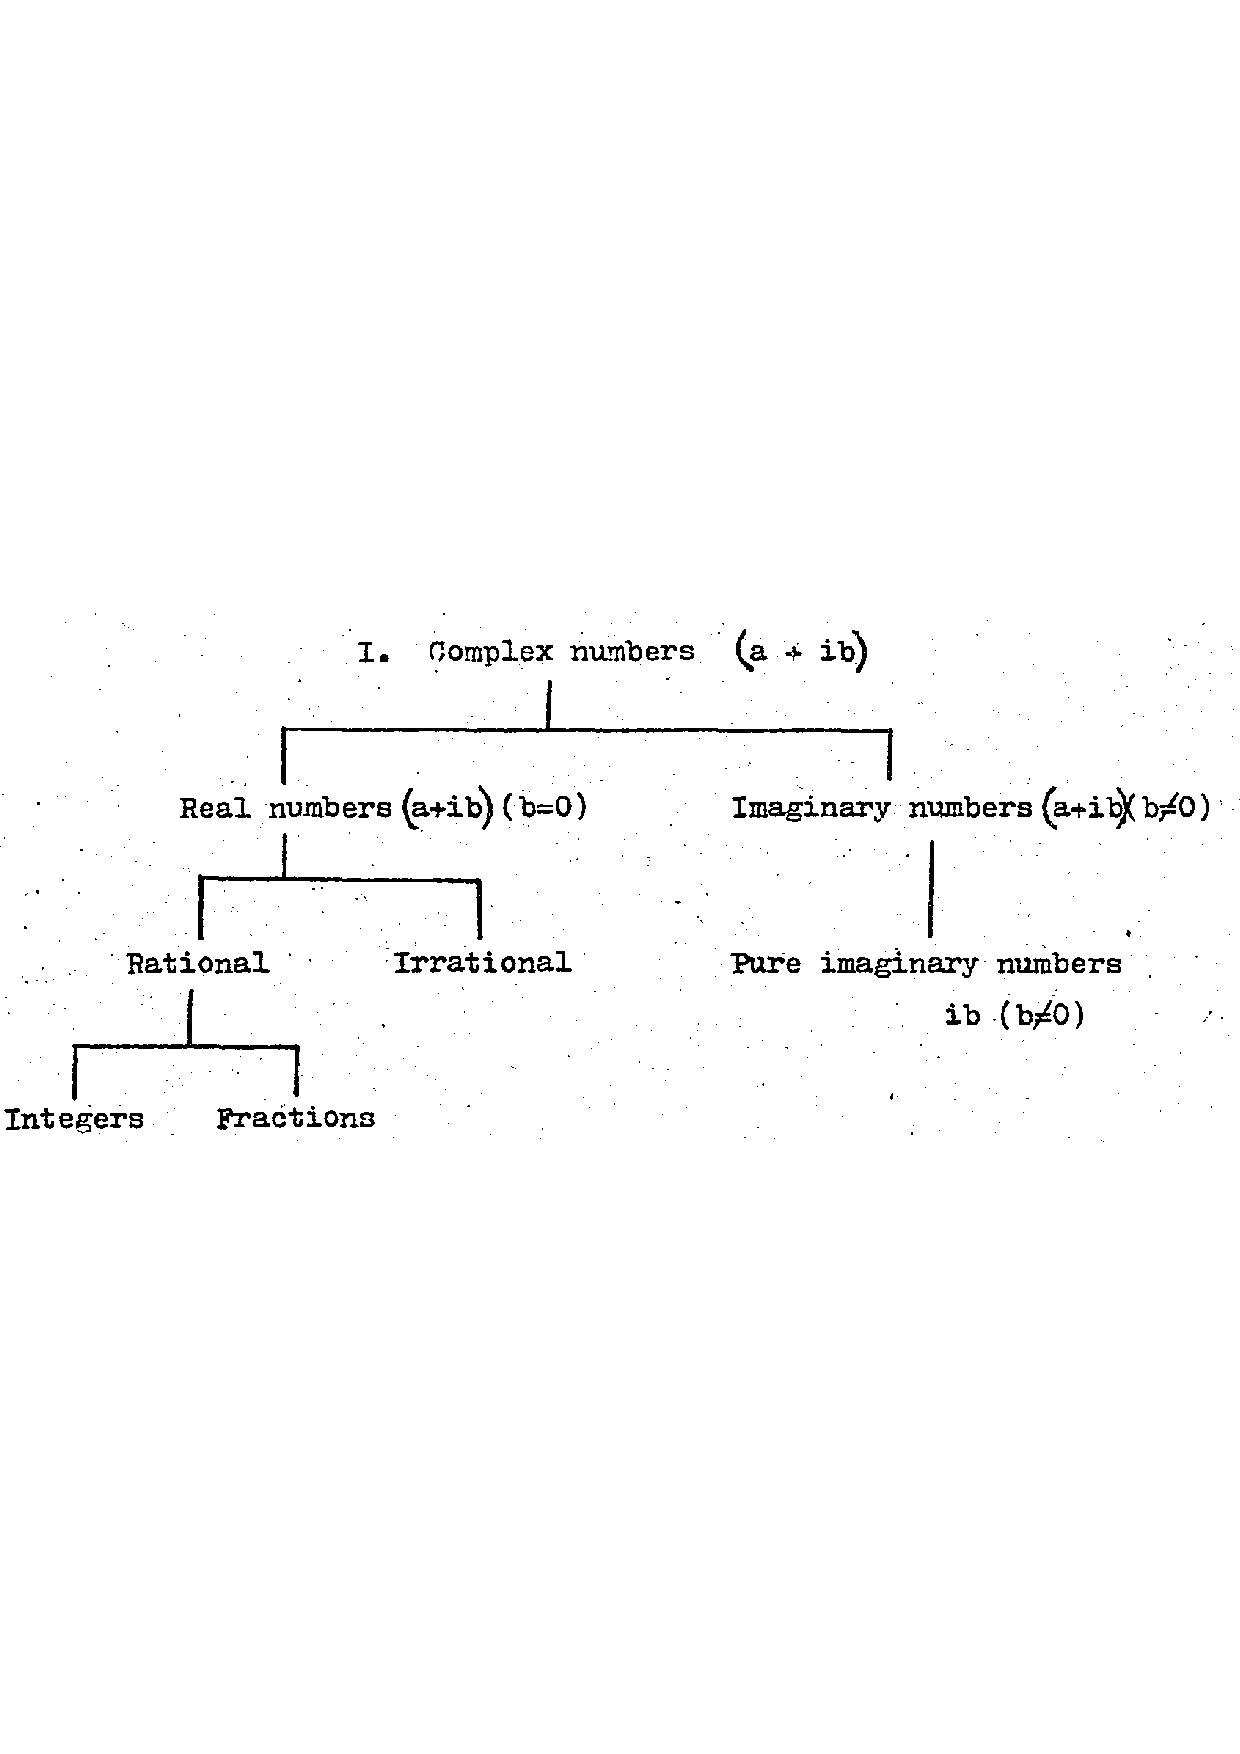
\includegraphics[width=0.9\textwidth]{images/SD-1-1p15A}
%	\caption{Classification of complex numbers}
%	\label{fig:classificationOfComplexNumbersA}
%\end{figure}

%\begin{center}
%\begin{tabular}{cc}
%\end{tabular}
%\end{center}

%\begin{exmp}
%\begin{hSolution}
%\end{hSolution}
%\end{exmp}

%\begin{hEnumerateAlpha}
%\end{hEnumerateAlpha}

%\begin{hEnumerateRoman}
%\end{hEnumerateRoman}

%$
%\begin{bmatrix}
%\end{bmatrix}
%$

%\frac{aaaa}{bbb}
%\frac{a_{n}}{b_{n}}
%\left( aaaa \right)
%\Longrightarrow

%\begin{multicols}{2}
%	bb
%\columnbreak
%	aa
%\end{multicols}
